\hypertarget{bullwinkle-socks}{%
\section{Bullwinkle socks}\label{bullwinkle-socks}}

\begin{figure}[!ht]
  \begin{adjustwidth}{-\oddsidemargin-1in}{-\rightmargin}
    \centering
    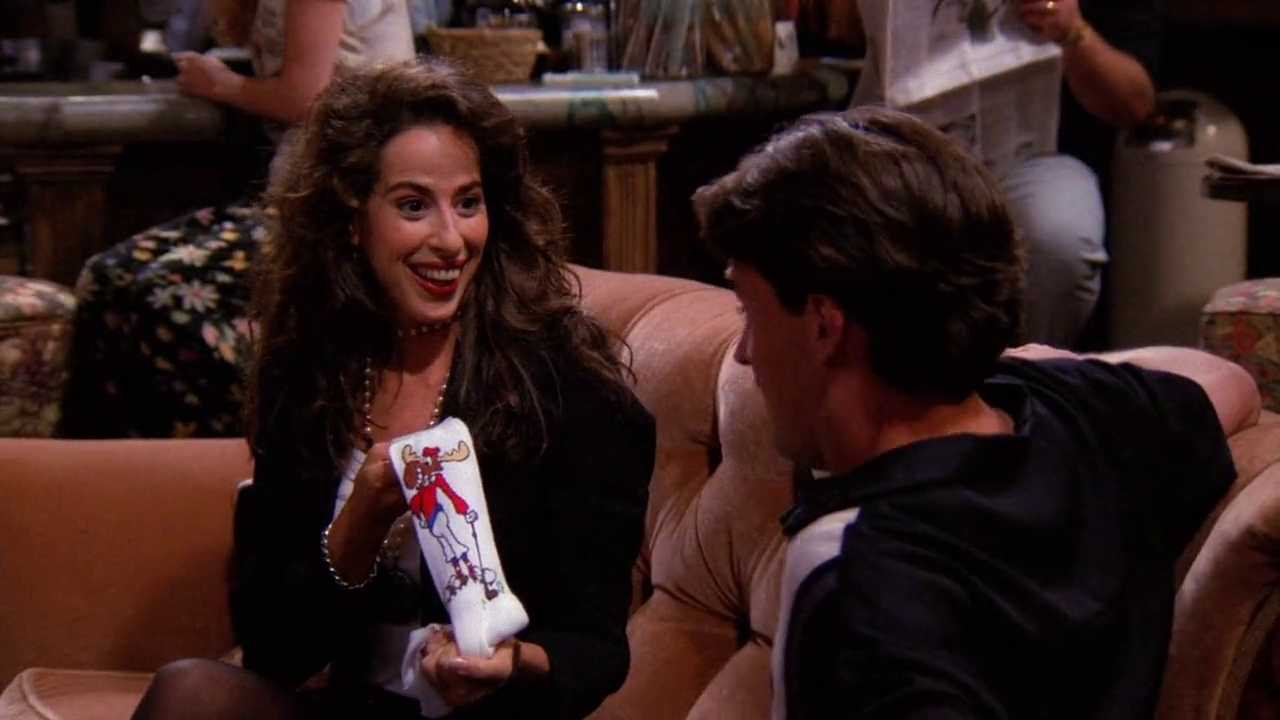
\includegraphics[trim={0 4cm 0 3cm,}, clip, width=\paperwidth]{./S01/img/5/bullwinkle-socks.png}
    \caption{Bullwinkle socks\label{fig:bullwinkle-socks}}
  \end{adjustwidth}
\end{figure}

\begin{tcolorbox}[enhanced,center upper,
    drop fuzzy shadow southeast, boxrule=0.3pt,
    lower separated=false,
    colframe=black!30!dialogoBorder,colback=white]
\begin{minipage}[c]{0.14\linewidth}
  \raisebox{\dimexpr-\height+\ht\strutbox\relax}{
    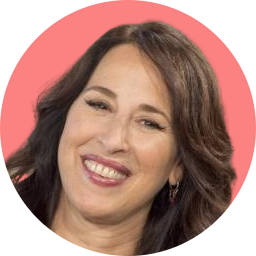
\includegraphics[width=1.5cm]{./assets/img/janice.png}
  }
   & \centering \scriptsize{Janice}
\end{minipage}
\hspace{.1mm}
\begin{minipage}[c]{0.8\linewidth}
  \textbf{- I got you... these.}\\
  - Comprei... isto.
\end{minipage}

\medskip
\begin{minipage}[c]{0.14\linewidth}
  \raisebox{\dimexpr-\height+\ht\strutbox\relax}{
    
\includegraphics[width=1.5cm]{./assets/img/chandler.png}
  }
   & \centering \scriptsize{Chandler}
\end{minipage}
\hspace{.1mm}
\begin{minipage}[c]{0.8\linewidth}
  \textbf{- Bullwinkle socks.}\\
  - Uma meia do Alceu.
\end{minipage}
\end{tcolorbox}

Para o dia dos namorados, Janice compra para Chandler meias do
\emph{Bullwinkle}, personagem de desenho animado, que junto com
\emph{Rocky}, estrelavam o programa \emph{The Rocky and Bullwinkle Show}
(1959). No Brasil a dupla ficou conhecida como Alceu (\emph{Bullwinkle})
e Dentinho (\emph{Rocky}).

\begin{figure}
  \centering
  \begin{tikzpicture}
    \node [inner sep=0pt] at (0,0) {
      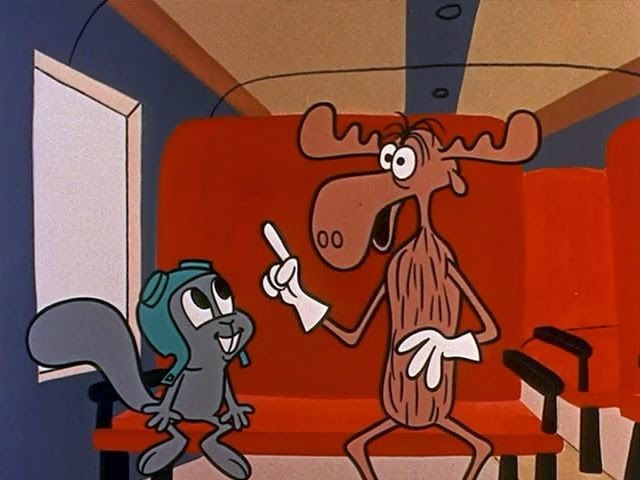
\includegraphics[width=0.6\textwidth,keepaspectratio]{./S01/img/5/rocky-bullwinkle.jpg}
    };
    \draw [white, rounded corners=\ClipSep, line width=\ClipSep]
    (current bounding box.north west) --
    (current bounding box.north east) --
    (current bounding box.south east) --
    (current bounding box.south west) -- cycle
    ;
    \end{tikzpicture}
    \caption{Rocky and Bullwinkle\label{fig:rocky-and-bullwinkle}}
\end{figure}

\hypertarget{referuxeancias}{%
\subsection{Referências}\label{referuxeancias}}

\begin{itemize}
\tightlist
\item
  \sloppy Fandom Wiki (Inglês). \url{https://rockyandbullwinkle.fandom.com/wiki/Bullwinkle_J._Moose}
\end{itemize}

\hypertarget{underdog}{%
\section{Underdog}\label{underdog}}

\begin{figure}[!ht]
  \begin{adjustwidth}{-\oddsidemargin-1in}{-\rightmargin}
    \centering
    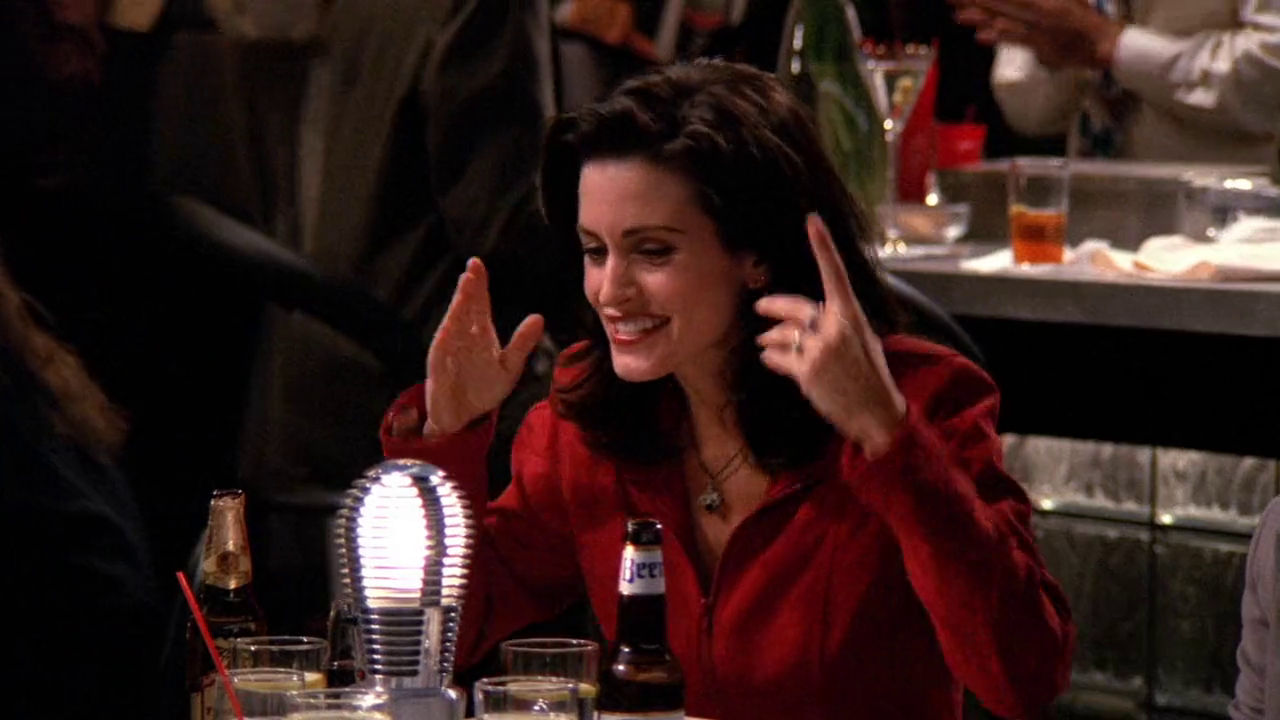
\includegraphics[trim={0 6.5cm 0 2.5cm,}, clip, width=\paperwidth]{./S01/img/5/underdog.png}
    \caption{Underdog\label{fig:underdog}}
  \end{adjustwidth}
\end{figure}

\begin{tcolorbox}[enhanced,center upper,
    drop fuzzy shadow southeast, boxrule=0.3pt,
    lower separated=false,
    colframe=black!30!dialogoBorder,colback=white]
\begin{minipage}[c]{0.14\linewidth}
  \raisebox{\dimexpr-\height+\ht\strutbox\relax}{
    
\includegraphics[width=1.5cm]{./assets/img/monica.png}
  }
   & \centering \scriptsize{Monica}
\end{minipage}
\hspace{.1mm}
\begin{minipage}[c]{0.8\linewidth}
  \textbf{- Something went wrong with Underdog, and they couldn't get his head to inflate.}\\
  - Aconteceu algo com o Vira-lata. E a cabeça dele não inflava.
\end{minipage}
\end{tcolorbox}

No ``encontro duplo'', Monica menciona o \emph{Underdog} (1964), desenho
animado americano protagonizado por um cão super-herói. O interessante
dessa cena é que Monica menciona algo que só vai ocorrer no episódio
\textbf{\textcolor{primarycolor}{S01E09 - Aquele em que o Underdog Escapa}},
quatro episódios mais tarde.

\begin{figure}
  \centering
  \begin{tikzpicture}
    \node [inner sep=0pt] at (0,0) {
      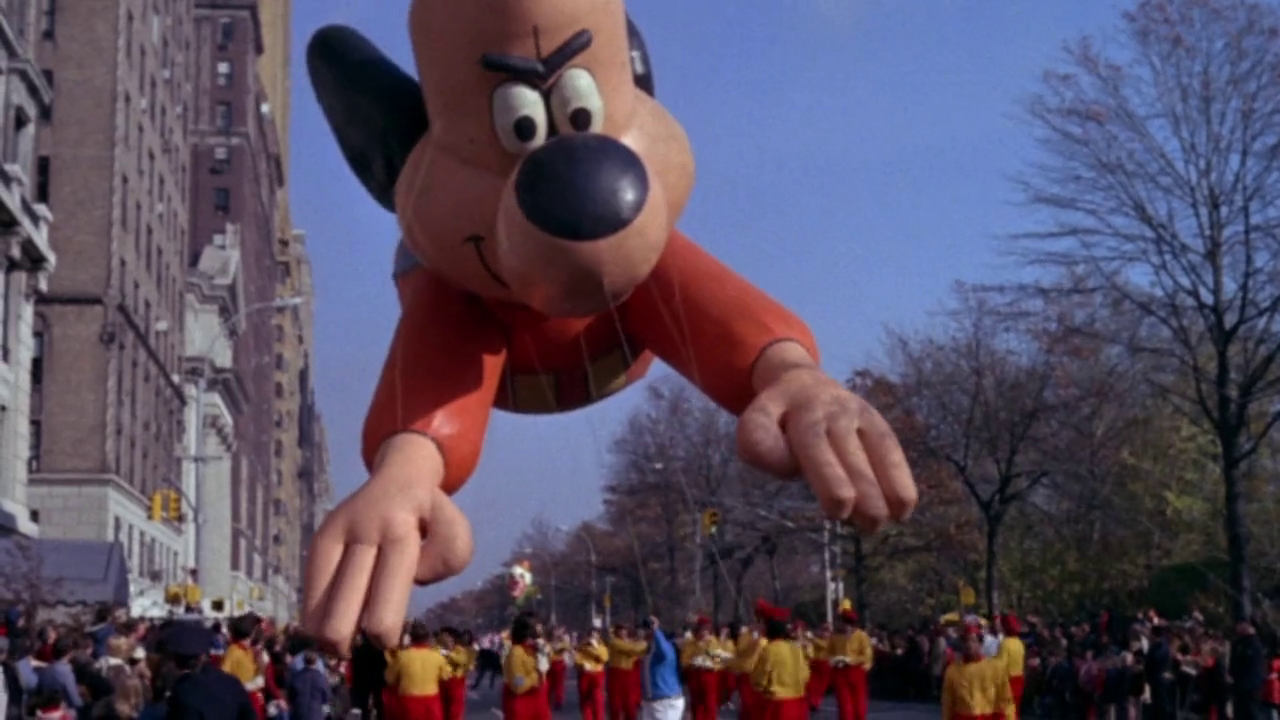
\includegraphics[width=0.7\textwidth,keepaspectratio]{./S01/img/5/underdog-s01e09.png}
    };
    \draw [white, rounded corners=\ClipSep, line width=\ClipSep]
    (current bounding box.north west) --
    (current bounding box.north east) --
    (current bounding box.south east) --
    (current bounding box.south west) -- cycle
    ;
    \end{tikzpicture}
    \caption{S01E09 - Aquele em que o Underdog Escapa\label{fig:s01-e09-aquele-em-que-o-underdog-escapa}}
\end{figure}

\hypertarget{referuxeancias-1}{%
\subsection{Referências}\label{referuxeancias-1}}

\begin{itemize}
\tightlist
\item
  \sloppy IMDB. \url{https://www.imdb.com/title/tt0060037/}
\item
  \sloppy Fandom Superhero Wiki. \url{https://superheroes.fandom.com/wiki/Underdog}
\end{itemize}

\hypertarget{cocktails-in-appalachia}{%
\section{Cocktails in Appalachia}\label{cocktails-in-appalachia}}

\begin{figure}[!ht]
  \begin{adjustwidth}{-\oddsidemargin-1in}{-\rightmargin}
    \centering
    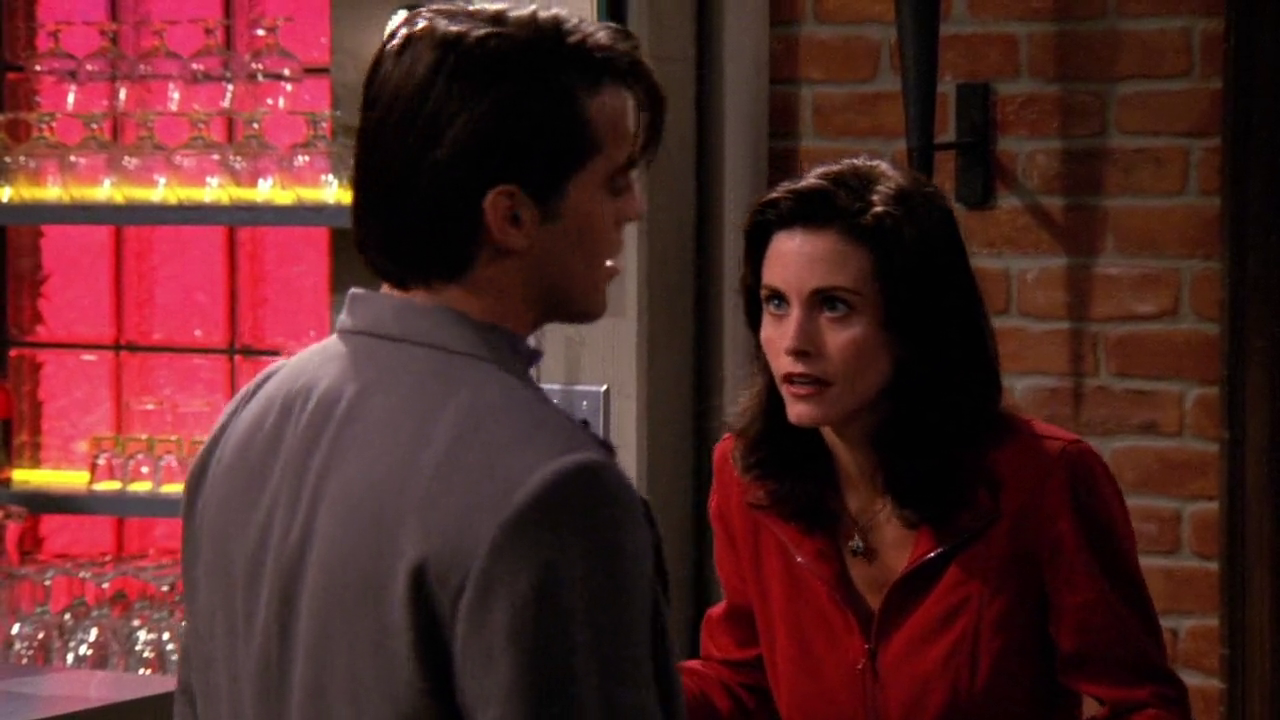
\includegraphics[trim={0 7cm 0 1cm,}, clip, width=\paperwidth]{./S01/img/5/cocktails-in-appalachia.png}
    \caption{Cocktails in Appalachia\label{fig:cocktails-in-appalachia}}
  \end{adjustwidth}
\end{figure}

\begin{tcolorbox}[enhanced,center upper,
    drop fuzzy shadow southeast, boxrule=0.3pt,
    lower separated=false,
    colframe=black!30!dialogoBorder,colback=white]
\begin{minipage}[c]{0.14\linewidth}
  \raisebox{\dimexpr-\height+\ht\strutbox\relax}{
    
\includegraphics[width=1.5cm]{./assets/img/monica.png}
  }
   & \centering \scriptsize{Monica}
\end{minipage}
\hspace{.1mm}
\begin{minipage}[c]{0.8\linewidth}
  \textbf{- Hello! Were we at the same table? It's like... Cocktails in Appalachia.}\\
  - Estamos na mesma mesa? Os dois estão pegando fogo!
\end{minipage}
\end{tcolorbox}

Abismada com o fato de Bob e Angela estarem se pegando, Monica menciona
que aquilo parecia \emph{Cocktails in Appalachia}. \emph{Appalachia} é
uma cidade do estado da Virgínia. O termo refere-se a esteriótipos do
local, que incluem incesto. Daí o termo usado por Monica, já que ela
pensa que os dois são irmãos.

\hypertarget{referuxeancias-2}{%
\subsection{Referências}\label{referuxeancias-2}}

\begin{itemize}
\tightlist
\item
  \sloppy MD Recruits Face Culture Shock in Appalachia - ABS News (Inglês). \url{https://abcnews.go.com/Health/story?id=5922943&page=1}
\end{itemize}
